\documentclass[11pt,a4paper]{article}
\usepackage[
    left=0.73in,
    right=0.73in,
    top=.8in,
    bottom=.50in,
    paperheight=11in,
    paperwidth=8.5in
]{geometry}

\begin{document}
% Cover Page
\pagenumbering{gobble}
\begin{center}
\textbf{
    \Large{ECE 543: Introduction to Digital Systems}
    \\~\\
    \large{Instructor: Bessam Zuhair Al Jewad, Ph.D.}
    \\[1.25in]
    \LARGE{Prelab \#3: The Universal Logic Gate}
    \\[0.62in]
    \large{Prepared for Himadri Basu (TA)\\~\\By Christopher Chin}
    \\[1.25in]
    \LARGE{Section 6}
    \\[1.25in]
    \Large{Department of Electrical and Computer Engineering\\
           University of New Hampshire}
    \\[1.25in]
    \Large{\today}
}
\end{center}
\clearpage
\pagenumbering{arabic}

% TOC
\tableofcontents
\pagebreak

% Pages
\section{Introduction}
The objective of this experiment is to become familiar with logic gates, particularly
the NAND gate, which will be used to implement the six basic logic functions.

\section{Equipment Required}
\begin{itemize}
    \item Global Specialties Design and Prototyping PB-505
    \item Wire leads
    \item 7400 TTL Integrated Circuit (1)
\end{itemize}

\section{Procedure}
\subsection{IC Diagrams}
\begin{figure}[h]
    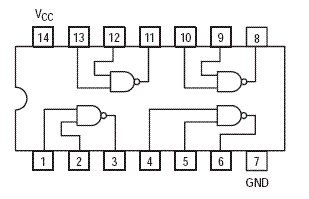
\includegraphics[width=5in]{IC7400.png}
    \caption{IC7400 Circuit Diagram}
\end{figure}
All internal gates are NAND gates.
Pin 14 is used as VCC$_{in}$. Pin 7 is GND.
Pin 1 and 2 are inputs to a logic gate that outputs to pin 3.
Pin 4 and 5 are inputs to a logic gate that outputs to pin 6.
Pin 13 and 12 are inputs to a logic gate that outputs to pin 11.
Pin 10 and 9 are inputs to a logic gate that outputs to pin 8.

\subsection{Work Done to Complete the Objective}
\subsection{Predicted Results and Discussion}
\section{References}

\end{document}
